\documentclass[10pt]{article}
\usepackage[margin=0.8in]{geometry}
\usepackage[utf8]{inputenc}
\usepackage[T1]{fontenc}
\usepackage[english]{babel}

\usepackage{fourier}
\usepackage{amsmath}
\usepackage{amssymb}
\usepackage{amsfonts}
\usepackage{amsthm}

\usepackage{graphicx}
\usepackage{float}
\usepackage{caption}
\usepackage{subcaption}

\usepackage{booktabs}

\usepackage{etoolbox}
\usepackage{siunitx}
\usepackage{parskip}
\usepackage{hyperref}
\usepackage{cite}

\usepackage{listings}
\usepackage{color}

\definecolor{codegreen}{rgb}{0,0.6,0}
\definecolor{codegray}{rgb}{0.5,0.5,0.5}
\definecolor{codepurple}{rgb}{0.58,0,0.82}
\definecolor{backcolour}{rgb}{0.95,0.95,0.92}

\lstdefinestyle{mystyle}{
    backgroundcolor=\color{backcolour},
    commentstyle=\color{codegreen},
    keywordstyle=\color{magenta},
    numberstyle=\tiny\color{codegray},
    stringstyle=\color{codepurple},
    basicstyle=\ttfamily\footnotesize,
    breakatwhitespace=false,
    breaklines=true,
    captionpos=b,
    keepspaces=true,
    numbers=left,
    numbersep=5pt,
    showspaces=false,
    showstringspaces=false,
    showtabs=false,
    tabsize=2,
    language=C++
}
\lstset{style=mystyle}

\newcommand{\code}[1]{\texttt{#1}}


\title{Assignment 2: Parallel Collatz Conjecture}
\author{Luca Lombardo \\ SPM Course a.a. 24/25}
\date{}

\begin{document}

\maketitle
\vspace{-1.5em}

\section{Sequential Baseline and Core Function}
The sequential implementation serves as our reference baseline. The \code{collatz\_steps(ull n)} function ensures correctness using \code{unsigned long long} types and overflow detection. For efficiency we use bitwise operations to handle parity checks and division. A key optimization targets power-of-two inputs ($n=2^k$): rather than iteratively dividing by two $k$ times, the function directly computes the result $k$ using the \code{\_\_builtin\_ctzll} intrinsic (count trailing zeros), significantly accelerating these cases. This implementation processes all input ranges through \code{find\_max\_steps\_in\_subrange}.

\section{Parallel Implementation Framework}
I built parallel versions using \code{std::thread} by partitioning input ranges into smaller tasks (chunks) that worker threads execute concurrently. For thread-safe aggregation of maximum step counts for each original range, I implemented a \code{RangeResult} structure containing \code{std::atomic<ull>} variables. Worker threads update these atomically via compare-and-swap (CAS) loops upon task completion. I chose this fine-grained approach to minimize synchronization bottlenecks during result updates. My implementations differ primarily in their task distribution (scheduling) strategy.

\subsection{Static Scheduling Strategies}
Static scheduling assigns tasks to threads deterministically before execution starts, with distribution patterns established upfront and fixed for the entire execution. I implemented three variants to compare their characteristics:
\begin{itemize}
    \item \textbf{Block:} Assigns large contiguous blocks per range to each thread. For example, with numbers 1-100 and 4 threads, thread 0 processes [1-25], thread 1 processes [26-50], and so on. It features low scheduling overhead but suffers from poor load balancing, especially for non-uniform workloads

    \item \textbf{Cyclic:} Assigns individual numbers round-robin. With the same example, thread 0 processes [1,5,9,...], thread 1 processes [2,6,10,...], etc. This offers fine-grained load balancing but can lead to suboptimal cache performance due to scattered memory accesses, as threads frequently access non-adjacent memory locations.

    \item \textbf{Block-Cyclic:} Divides work into blocks of a specified \code{chunk\_size}, which are then assigned cyclically using a global block index computed across all input ranges. With \code{chunk\_size=4}, thread 0 processes [1-4,17-20,...], thread 1 processes [5-8,21-24,...], etc. This strategy aims to balance load better than pure Block while potentially improving cache locality compared to pure Cyclic.
\end{itemize}
Static schedulers are typically suitable for predictable, balanced workloads due to their minimal runtime overhead. The key advantage is that no synchronization is required during execution since work distribution is determined entirely in advance. For the Collatz problem specifically, the varying computation cost of different numbers (e.g., powers of 2 vs. odd numbers) makes the choice of static scheduling strategy particularly important.


\subsection{Dynamic Scheduling Strategies}
For workloads with variable task execution times like Collatz computation, I found dynamic scheduling strategies typically outperform static assignments. Since they let idle threads grab new tasks as they become available, they can significantly improve load balancing. I explored three dynamic scheduling approaches:

\begin{enumerate}
    \item \textbf{Centralized Task Queue:} I implemented this straightforward approach using a single shared queue (my \code{TaskQueue} class) protected by a \code{std::mutex} and a \code{std::condition\_variable} to efficiently manage thread signaling. This approach was simple to implement and provided natural load balancing since any free thread could take the next task whenever it became available. However, there is a potential limitation: the single mutex protecting the queue can become a bottleneck when many threads are competing for access, limiting scalability as thread count increased.

    \item \textbf{Work-Stealing with Mutex-Based Deques:} To address the scalability issues in my centralized approach, I decentralized task management by giving each thread its own deque (my \code{WorkStealingQueue} class). Threads primarily work with their local queue (using LIFO operations for better cache locality) but can "steal" tasks (using FIFO operations) from other threads when they become idle. This significantly reduced contention compared to my centralized queue implementation and scaled much better with higher thread counts. The LIFO access pattern for local work also improved cache locality for better performance.

    \item \textbf{Lock-Free Work-Stealing:} Pushing for even better performance, I attempted using exclusively atomic operations and carefully controlled memory ordering to eliminate mutexes entirely. This approach theoretically offers the highest performance by completely avoiding lock contention, but I found it extremely difficult to implement correctly. Managing atomics and memory ordering proved challenging, especially with edge cases like concurrent operations on nearly-empty deques where multiple threads might try to take the last task simultaneously.
\end{enumerate}

I spent considerable time trying to implement a lock-free work-stealing deque based on Chase-Lev principles. Despite focusing on atomic interactions and memory synchronization, my implementation was unstable - it often deadlocked or hung during testing. I noticed its behavior changed with subtle timing variations or even debugging prints, classic signs of complex race conditions. Given these challenges and the project timeframe, I made a practical decision to focus on ensuring robust implementations of the other two approaches. I fully implemented, tested and benchmarked both the Centralized Task Queue and Mutex-Based Work-Stealing approaches for this report.

\section{Theoretical Performance Analysis}

I applied the Work-Span model to estimate the parallelism in my benchmark workloads. For this analysis, I approximated Work (W) as the total Collatz steps across all numbers, and Span (S) as the maximum steps for any single number. The theoretical Parallelism $P = W/S$ indicates the maximum possible speedup we could achieve in an ideal scenario, neglecting all practical overheads.

\begin{table}[H]
    \centering
    \caption{Theoretical Work-Span Analysis Results for Benchmark Workloads.}
    \label{tab:theoretical}
    \begin{tabular}{@{}l S[table-format=9.0] S[table-format=3.0] S[table-format=6.1]@{}}
        \toprule
        Workload Description                                                      & {Work (W)} & {Span (S)} & {Parallelism (P=W/S)} \\ \midrule
        Medium Balanced (1-100k)                                                  & 10753840   & 350        & 30725.3               \\
        Large Balanced (1-1M)                                                     & 131434424  & 524        & 250829.0              \\
        Unbalanced Mix (Small, Large, Medium)                                     & 66057430   & 448        & 147450.0              \\
        Many Small Uniform Ranges (500x1k)                                        & 62134795   & 448        & 138694.0              \\
        Ranges Around Powers of 2 (2\textasciicircum{}8 to 2\textasciicircum{}20) & 1271514    & 363        & 3502.8                \\
        Extreme Imbalance with Isolated Expensive Calculations                    & 1113876    & 685        & 1626.1                \\ \bottomrule
    \end{tabular}
\end{table}

My analysis in Table \ref{tab:theoretical} shows that theoretical Parallelism ($P$) varies significantly across workloads, primarily driven by the large differences in total Work (W). I found that workloads processing substantially more numbers (e.g., "Large Balanced", "Unbalanced Mix") naturally have orders of magnitude more total work. Since the Span (S), determined by the single longest sequence, varies relatively little (within a factor of $\approx$2 in this case), I observed that the $P=W/S$ ratio largely mirrors the scale of W.

Therefore, in my analysis, while workloads like "Large Balanced" show extremely high theoretical parallelism ($P \approx 250k$), indicating vast potential for parallel execution limited mainly by processor count, workloads like "Extreme Imbalance" ($P \approx 1.6k$) are theoretically limited sooner. I found this isn't necessarily because their critical path is intrinsically problematic relative to the type of work, but because the total amount of work (W) is much smaller compared to their Span (S). This led me to conclude that achieving high speedups on smaller workloads might be challenging even theoretically, before considering any practical overheads in my implementations.


\section{Experimental Performance Analysis}

The parallel implementations were benchmarked on a dual-socket system with two Intel Xeon Gold 5318Y CPUs, offering 48 physical cores (96 logical threads) in a NUMA architecture\footnote{We will see that this architecture affects significantly the scalability of the implementations, that are NUMA-unaware}. The system runs Ubuntu 22.04 with 1TB RAM, and all code was compiled using GCC 11.4.0 with \code{-std=c++17 -O3 -pthread} options. Execution times reported are the median of 10 samples (each with 50 iterations) to ensure measurement reliability. Strong speedup is calculated relative to the optimized sequential baseline. Tests explored thread counts up to 96 and chunk sizes ranging from 16 to 1024.

\subsection{Static vs. Dynamic Scheduling Speedup}
The performance comparison between static and dynamic schedulers highlights the importance of workload characteristics and the underlying hardware architecture. Figure \ref{fig:speedup_comparison_grid} presents the speedup achieved on four representative workloads, utilizing the empirically determined optimal chunk size for chunk-dependent schedulers (Static Block-Cyclic, Dynamic TaskQueue, Dynamic WorkStealing) for each specific workload.

\begin{figure}[H]
    \centering
    \begin{subfigure}[b]{0.49\textwidth}
        \centering
        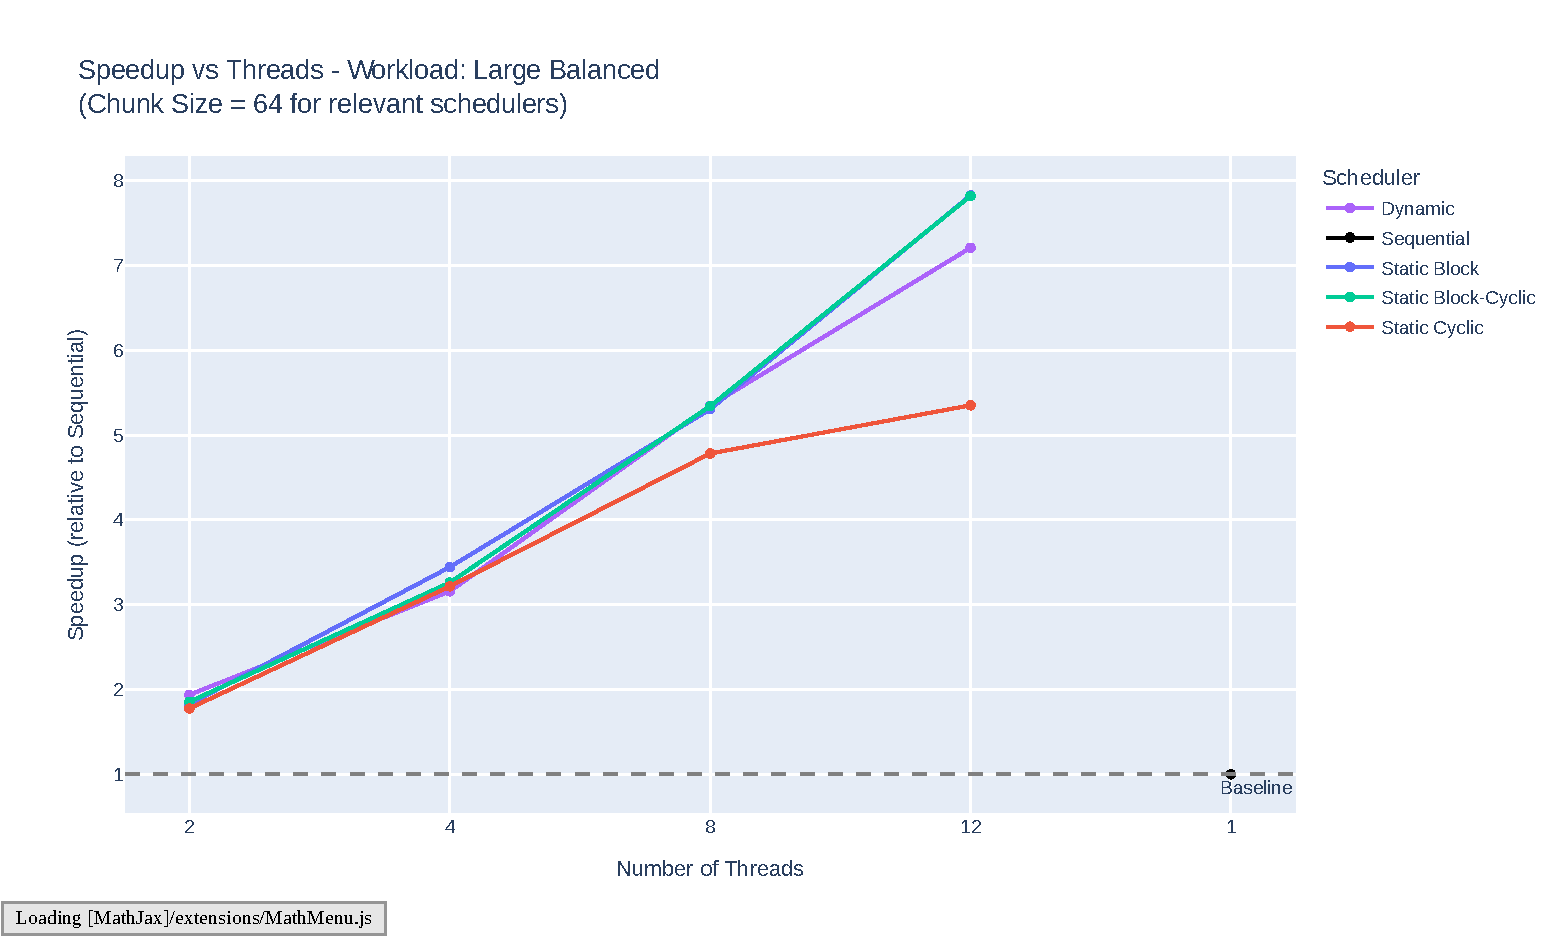
\includegraphics[width=\textwidth]{../results/plots/speedup_vs_threads/speedup_vs_threads_W1.pdf}
        \caption{Large Balanced (1-1M) - Optimal Chunk 1024}
        \label{fig:speedup_large_balanced}
    \end{subfigure}
    \hfill
    \begin{subfigure}[b]{0.49\textwidth}
        \centering
        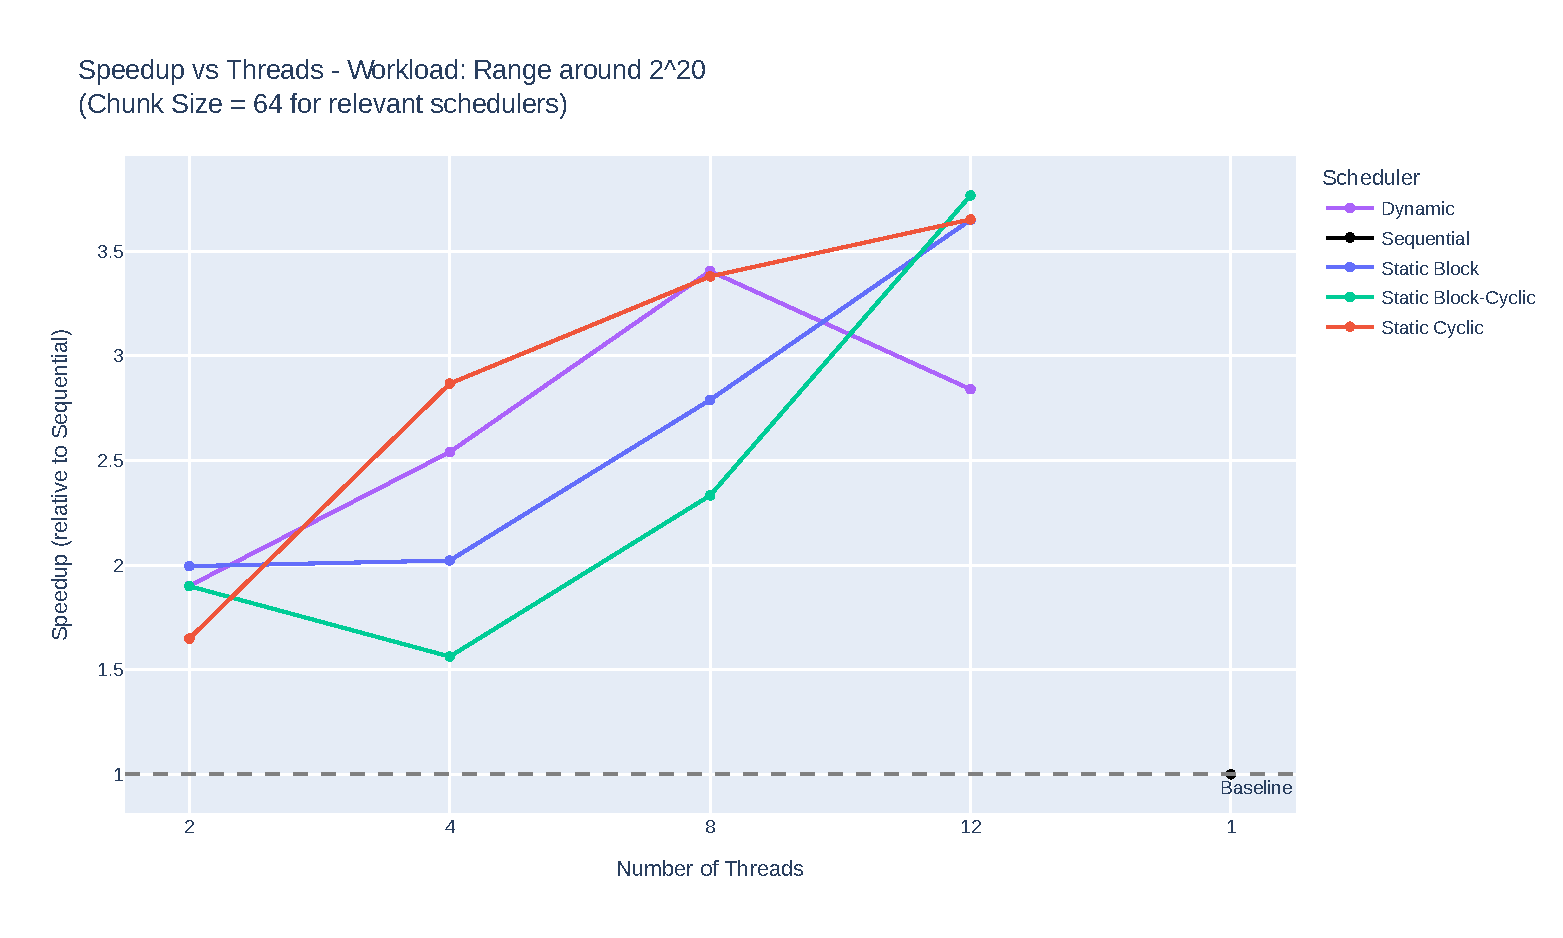
\includegraphics[width=\textwidth]{../results/plots/speedup_vs_threads/speedup_vs_threads_W5.pdf}
        \caption{Extreme Imbalance - Optimal Chunk 256}
        \label{fig:speedup_extreme_imbalance}
    \end{subfigure}

    \vspace{1em}

    \begin{subfigure}[b]{0.49\textwidth}
        \centering
        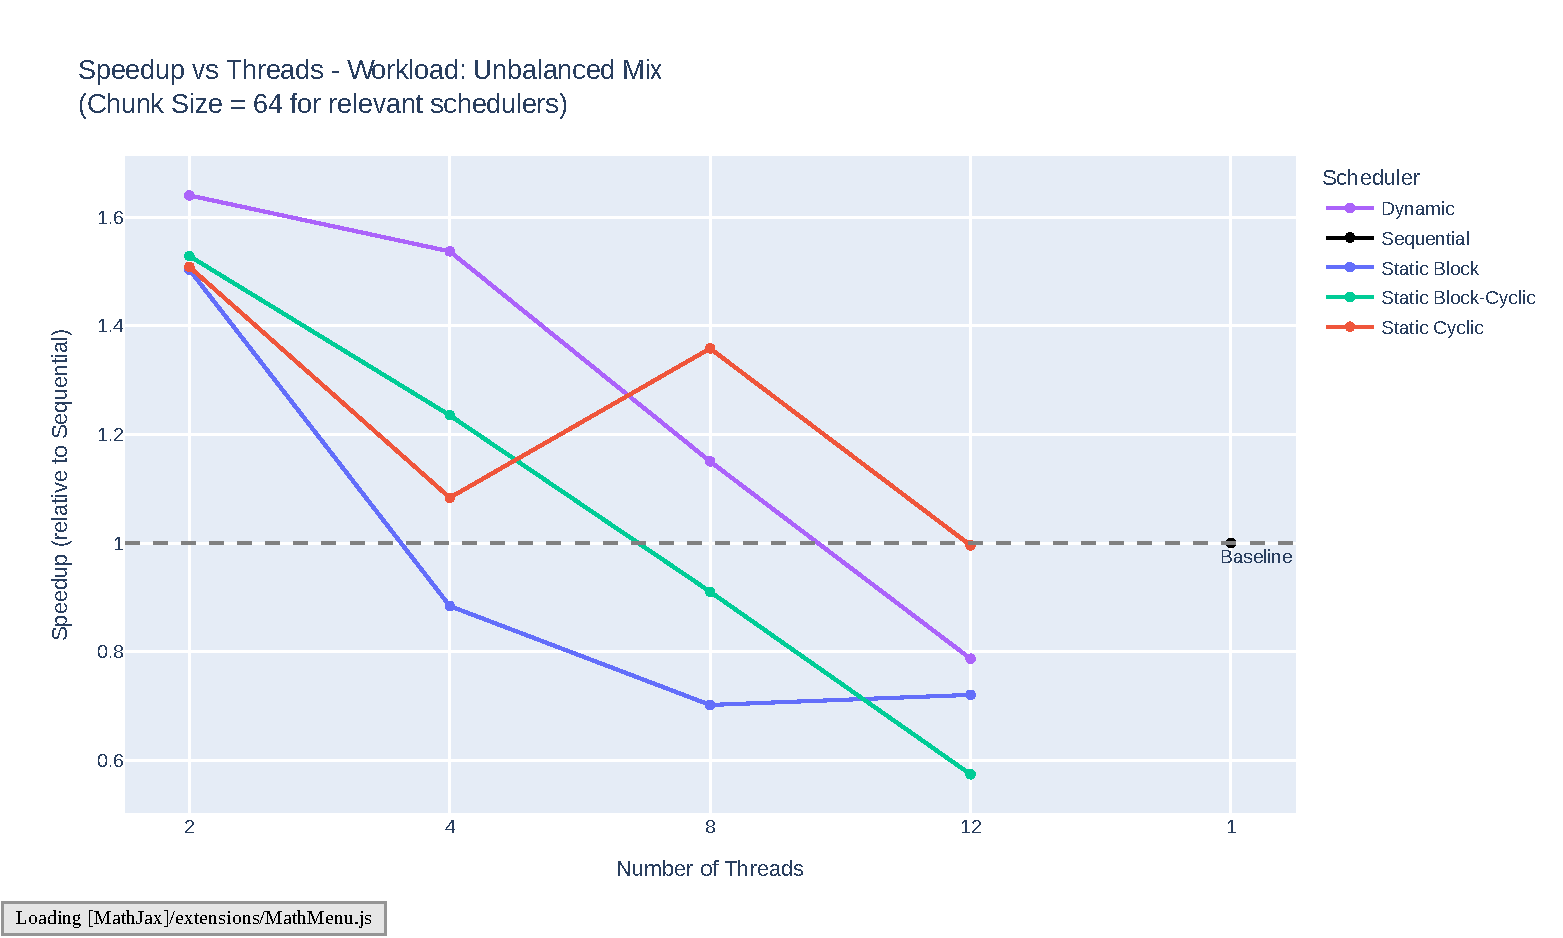
\includegraphics[width=\textwidth]{../results/plots/speedup_vs_threads/speedup_vs_threads_W2.pdf}
        \caption{Unbalanced Mix (Small, Large, Medium)}
        \label{fig:speedup_unbalanced_mix}
    \end{subfigure}
    \hfill
    \begin{subfigure}[b]{0.49\textwidth}
        \centering
        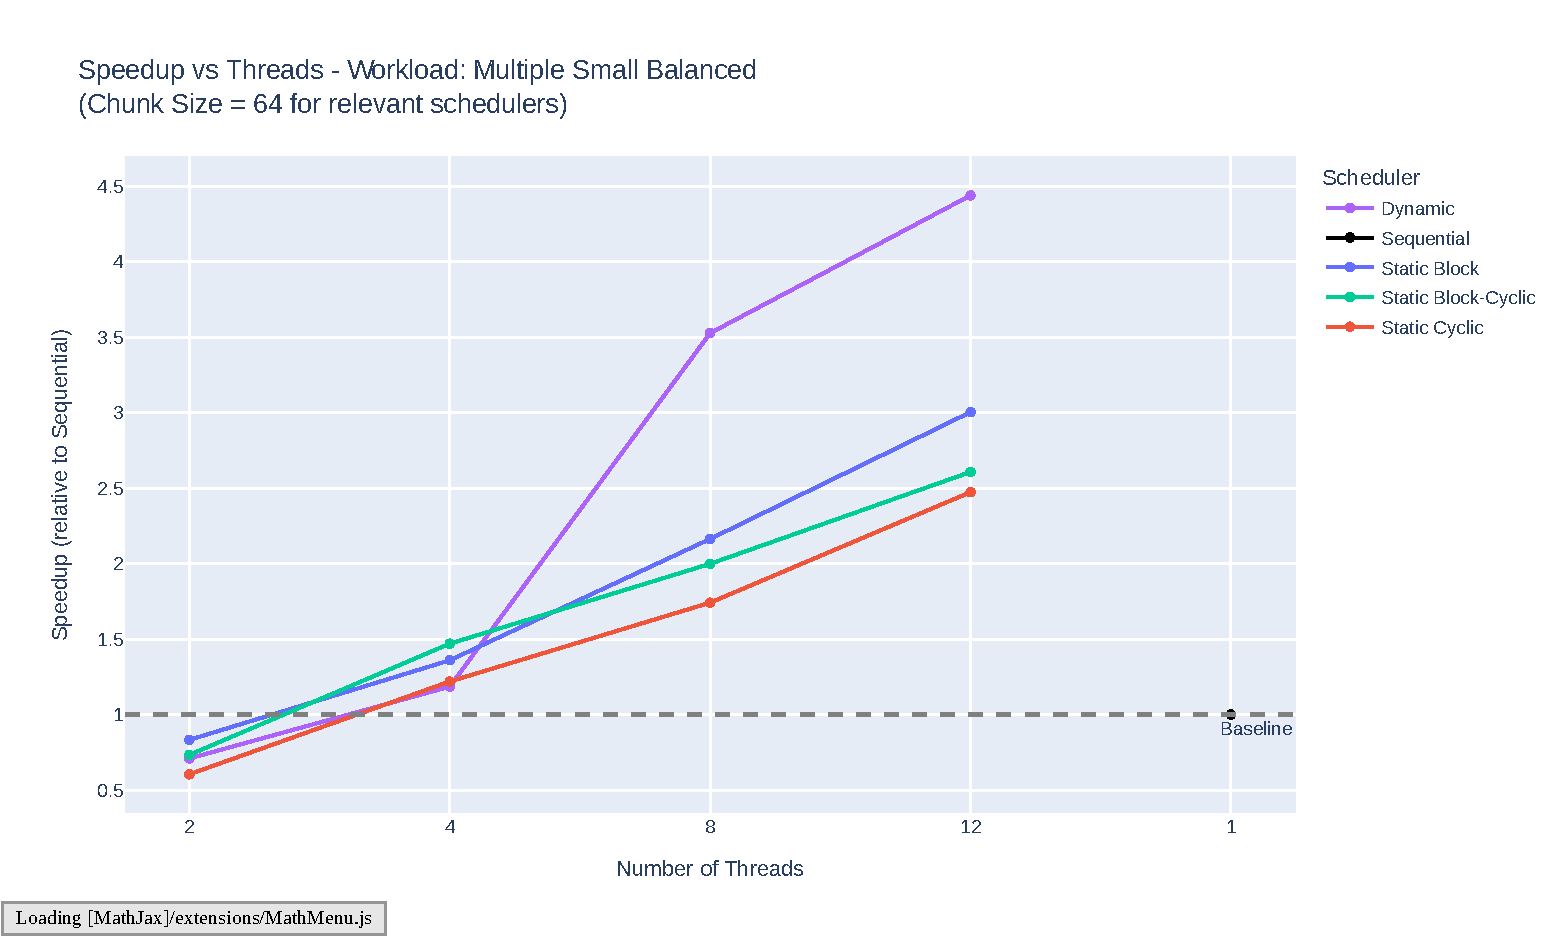
\includegraphics[width=\textwidth]{../results/plots/speedup_vs_threads/speedup_vs_threads_W3.pdf}
        \caption{Many Small Uniform Ranges (500x1k)}
        \label{fig:speedup_many_small}
    \end{subfigure}

    \caption{Speedup vs. Threads for selected workloads (Chunked schedulers use optimal chunk size per workload)}
    \label{fig:speedup_comparison_grid}
\end{figure}

For balanced workloads with substantial computation (Fig \ref{fig:speedup_large_balanced}), well-tuned static and dynamic schedulers perform nearly identically, achieving excellent speedup (21-22x) at 48 threads. This indicates that when computation is uniform, scheduler overhead differences become negligible compared to the actual computation time. The "Extreme Imbalance" workload (Fig \ref{fig:speedup_extreme_imbalance}) reveals a counter-intuitive result: static schedulers (particularly Block-Cyclic) outperform dynamic approaches. This suggests that for workloads with many extremely short tasks, the overhead of dynamic scheduling mechanisms (mutex contention, deque operations) becomes significant relative to task execution time. Static approaches benefit from their lower scheduling overhead despite potentially imperfect load distribution. Similar patterns appear in mixed workloads (Fig \ref{fig:speedup_unbalanced_mix}, \ref{fig:speedup_many_small}).

A critical observation is the performance degradation beyond 48 threads across all implementations. This clearly demonstrates the impact of the system's NUMA architecture, where cross-socket communication penalties begin to outweigh the benefits of additional threads.

\subsection{Impact of Chunk Size}
The chunk size parameter mediates the trade-off between scheduling overhead (favoring larger chunks) and load balancing granularity (favoring smaller chunks). Figure \ref{fig:chunk_impact_combined} illustrates this by comparing the speedup of Dynamic TaskQueue, Dynamic WorkStealing, and Static Block-Cyclic across various chunk sizes for both the "Large Balanced" and "Extreme Imbalance" workloads.

\begin{figure}[H]
    \centering
    \begin{subfigure}[b]{0.49\textwidth}
        \centering
        \includegraphics[width=\textwidth]{../results/plots/dynamic_taskqueue_chunk_comparison/dynamic_taskqueue_chunks_W1.pdf}
        \caption{Dynamic TaskQueue: Large Balanced}
        \label{fig:chunk_impact_dynamic_balanced_TQ}
    \end{subfigure}
    \hfill
    \begin{subfigure}[b]{0.49\textwidth}
        \centering
        \includegraphics[width=\textwidth]{../results/plots/dynamic_taskqueue_chunk_comparison/dynamic_taskqueue_chunks_W5.pdf}
        \caption{Dynamic TaskQueue: Extreme Imbalance}
        \label{fig:chunk_impact_dynamic_imbalance_TQ}
    \end{subfigure}

    \vspace{0.5em}

    \begin{subfigure}[b]{0.49\textwidth}
        \centering
        \includegraphics[width=\textwidth]{../results/plots/dynamic_workstealing_chunk_comparison/dynamic_workstealing_chunks_W1.pdf}
        \caption{Dynamic WorkStealing: Large Balanced}
        \label{fig:chunk_impact_dynamic_balanced_WS}
    \end{subfigure}
    \hfill
    \begin{subfigure}[b]{0.49\textwidth}
        \centering
        \includegraphics[width=\textwidth]{../results/plots/dynamic_workstealing_chunk_comparison/dynamic_workstealing_chunks_W5.pdf}
        \caption{Dynamic WorkStealing: Extreme Imbalance}
        \label{fig:chunk_impact_dynamic_imbalance_WS}
    \end{subfigure}

    \vspace{0.5em}

    \begin{subfigure}[b]{0.49\textwidth}
        \centering
        \includegraphics[width=\textwidth]{../results/plots/static_block_cyclic_chunk_comparison/static_block_cyclic_chunks_W1.pdf}
        \caption{Static Block-Cyclic: Large Balanced}
        \label{fig:chunk_impact_sbc_balanced}
    \end{subfigure}
    \hfill
    \begin{subfigure}[b]{0.49\textwidth}
        \centering
        \includegraphics[width=\textwidth]{../results/plots/static_block_cyclic_chunk_comparison/static_block_cyclic_chunks_W5.pdf}
        \caption{Static Block-Cyclic: Extreme Imbalance}
        \label{fig:chunk_impact_sbc_imbalance}
    \end{subfigure}

    \caption{Impact of Chunk Size on Scheduler Speedup vs. Threads for both Static and Dynamic approaches.}
    \label{fig:chunk_impact_combined}
\end{figure}

Static Block-Cyclic (Figures \ref{fig:chunk_impact_sbc_balanced} and \ref{fig:chunk_impact_sbc_imbalance}) demonstrates notable resilience to chunk size variation, particularly with balanced workloads. Its performance overhead is primarily from initial distribution, not runtime scheduling. In contrast, dynamic schedulers (TaskQueue in Figures \ref{fig:chunk_impact_dynamic_balanced_TQ} and \ref{fig:chunk_impact_dynamic_imbalance_TQ}, and WorkStealing in Figures \ref{fig:chunk_impact_dynamic_balanced_WS} and \ref{fig:chunk_impact_dynamic_imbalance_WS}) show higher sensitivity to chunk size selection. For balanced workloads, larger chunks minimize overhead in both TaskQueue and WorkStealing approaches. However, with imbalanced workloads, medium-sized chunks provide better load distribution.

\subsection{Performance Heatmaps}
Heatmaps provide a comprehensive visualization of performance across the entire tested parameter space of thread count and chunk size. Figure \ref{fig:heatmaps_all} shows these heatmaps for the Dynamic TaskQueue, Dynamic WorkStealing, and Static Block-Cyclic schedulers on both balanced and imbalanced workloads.

\begin{figure}[H]
    \centering
    \begin{subfigure}[b]{0.32\textwidth}
        \centering
        \includegraphics[width=\textwidth]{../results/plots/speedup_heatmaps_chunk_vs_threads/heatmap_speedup_dynamic_taskqueue_W1.pdf}
        \caption{Dyn TQ: Large Balanced}
        \label{fig:heatmap_dynamic_TQ_balanced}
    \end{subfigure}
    \hfill
    \begin{subfigure}[b]{0.32\textwidth}
        \centering
        \includegraphics[width=\textwidth]{../results/plots/speedup_heatmaps_chunk_vs_threads/heatmap_speedup_dynamic_workstealing_W1.pdf}
        \caption{Dyn WS: Large Balanced}
        \label{fig:heatmap_dynamic_WS_balanced}
    \end{subfigure}
    \hfill
    \begin{subfigure}[b]{0.32\textwidth}
        \centering
        \includegraphics[width=\textwidth]{../results/plots/speedup_heatmaps_chunk_vs_threads/heatmap_speedup_static_block_cyclic_W1.pdf}
        \caption{Static BC: Large Balanced}
        \label{fig:heatmap_sbc_balanced}
    \end{subfigure}

    \vspace{0.5em}

    \begin{subfigure}[b]{0.32\textwidth}
        \centering
        \includegraphics[width=\textwidth]{../results/plots/speedup_heatmaps_chunk_vs_threads/heatmap_speedup_dynamic_taskqueue_W5.pdf}
        \caption{Dyn TQ: Extreme Imbalance}
        \label{fig:heatmap_dynamic_TQ_imbalance}
    \end{subfigure}
    \hfill
    \begin{subfigure}[b]{0.32\textwidth}
        \centering
        \includegraphics[width=\textwidth]{../results/plots/speedup_heatmaps_chunk_vs_threads/heatmap_speedup_dynamic_workstealing_W5.pdf}
        \caption{Dyn WS: Extreme Imbalance}
        \label{fig:heatmap_dynamic_WS_imbalance}
    \end{subfigure}
    \hfill
    \begin{subfigure}[b]{0.32\textwidth}
        \centering
        \includegraphics[width=\textwidth]{../results/plots/speedup_heatmaps_chunk_vs_threads/heatmap_speedup_static_block_cyclic_W5.pdf}
        \caption{Static BC: Extreme Imbalance}
        \label{fig:heatmap_sbc_imbalance}
    \end{subfigure}
    \caption{Speedup Heatmaps for Balanced (top row) and Imbalanced (bottom row) Workloads (Chunk Size vs. Number of Threads).}
    \label{fig:heatmaps_all}
\end{figure}

For the "Large Balanced" workload (Figures \ref{fig:heatmap_dynamic_TQ_balanced}, \ref{fig:heatmap_dynamic_WS_balanced}, and \ref{fig:heatmap_sbc_balanced}), all three schedulers exhibit a broad region of optimal performance (brightest yellow areas). This region typically spans medium-to-large chunk sizes (256-1024) and moderate-to-high thread counts within a single socket ($\approx$30-48 threads). This visually confirms that multiple parameter combinations yield good results when the workload is regular.

Conversely, for the "Extreme Imbalance" workload (Figures \ref{fig:heatmap_dynamic_TQ_imbalance}, \ref{fig:heatmap_dynamic_WS_imbalance}, and \ref{fig:heatmap_sbc_imbalance}), the optimal performance region is much narrower and located differently. High speedup is concentrated at lower thread counts (roughly 8-16 threads) and requires smaller intermediate chunk sizes (typically 64-256, sometimes up to 512). The heatmaps also visually suggest that Static Block-Cyclic (Fig \ref{fig:heatmap_sbc_imbalance}) achieves a slightly higher peak speedup (brighter spot) within its optimal zone compared to the dynamic schedulers (Fig \ref{fig:heatmap_dynamic_TQ_imbalance}, \ref{fig:heatmap_dynamic_WS_imbalance}) for this specific challenging workload.

\end{document}
